\documentclass[tikz,border=10pt]{standalone}
\usepackage{amsmath}
\usepackage{amssymb}
\usepackage{tikz}
\usetikzlibrary{arrows.meta,calc}

\definecolor{figazul}{RGB}{2,132,199}
\definecolor{figrojo}{RGB}{220,38,38}
\definecolor{figverde}{RGB}{22,163,74}
\definecolor{figmorado}{RGB}{124,58,237}

\begin{document}
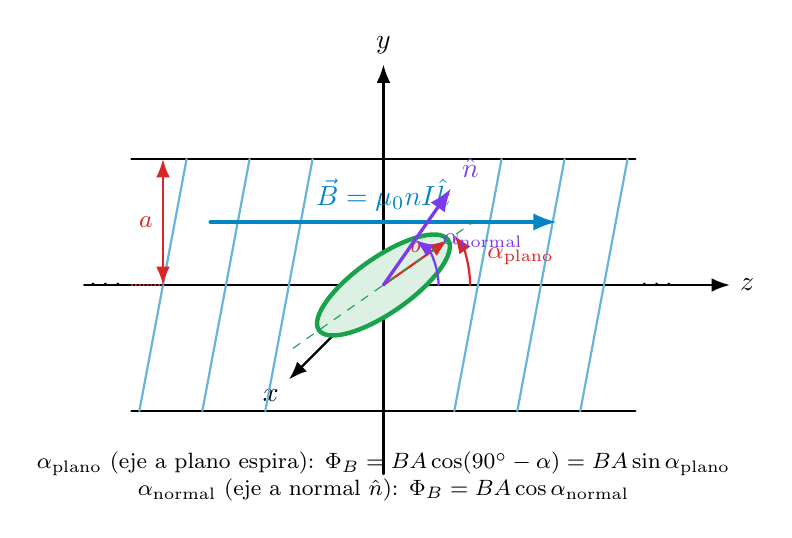
\begin{tikzpicture}[>=Latex, line cap=round, line join=round]
  % Eje longitudinal z del solenoide (horizontal hacia la derecha)
  \draw[->, thick] (-3.8, 0) -- (4.4, 0) node[right] {$z$};
  \draw[->, thick] (0, -2.4) -- (0, 2.8) node[above] {$y$};
  \node[below left] at (0,0) {$O$};

  % Eje x saliente
  \draw[->, thick] (0, 0) -- (-1.2, -1.2) node[below left] {$x$};

  % Solenoide ideal muy largo de radio a = 1.6
  % Contornos superior e inferior
  \draw[thick] (-3.2, 1.6) -- (3.2, 1.6);
  \draw[thick] (-3.2, -1.6) -- (3.2, -1.6);
  \node at (-3.5, 0) {$\cdots$};
  \node at (3.5, 0) {$\cdots$};

  % Espiras del solenoide (arcos cilíndricos continuos)
  \foreach \z in {-2.8, -2.0, -1.2, 1.2, 2.0, 2.8} {
    \draw[thick, color=figazul!60] (\z-0.3, -1.6) -- (\z+0.3, 1.6);
  }

  % Campo magnético B del solenoide a lo largo de +z
  \draw[->, very thick, color=figazul] (-2.2, 0.8) -- (2.2, 0.8) node[above, midway, color=figazul] {$\vec{B} = \mu_0 n I \hat{k}$};

  % Cota del radio a del solenoide (en rojo)
  \draw[<->, thick, color=figrojo] (-2.8, 0) -- (-2.8, 1.6) node[midway, left, color=figrojo, font=\small] {$a$};
  \draw[densely dotted, thin, color=figrojo] (-3.2, 0) -- (-2.8, 0);

  % Espira interior de radio b = 1.0, inclinada
  % Orientación: plano a 35° respecto a la horizontal
  \begin{scope}[rotate=35]
    % Elipse que representa la espira circular vista en perspectiva
    \draw[ultra thick, color=figverde, fill=figverde!15] (0, 0) ellipse (1.0 and 0.35);

    % Cota de radio b de la espira
    \draw[->, thick, color=figrojo] (0, 0) -- (1.0, 0);
    \node[above, color=figrojo, font=\footnotesize] at (0.5, 0) {$b$};

    % Trazo auxiliar del plano de la espira
    \draw[dashed, thin, color=figverde] (-1.4, 0) -- (1.4, 0);
  \end{scope}

  % Vector normal n_hat perpendicular al plano (a 35° + 90° = 125° o apuntando hacia +z a 55°)
  % Normal con componente +z: ángulo 90° - 35° = 55°
  \draw[->, very thick, color=figmorado] (0, 0) -- (55:1.5) node[above right, color=figmorado] {$\hat{n}$};

  % Ángulo 1 (alpha_plano = 35°): entre eje horizontal z y el plano de la espira
  \draw[->, thick, color=figrojo] (1.1, 0) arc (0:35:1.1);
  \node[right, color=figrojo, font=\small] at (17:1.25) {$\alpha_{\text{plano}}$};

  % Ángulo 2 (alpha_normal = 55° = 90° - alpha_plano): entre eje z y el vector normal n_hat
  \draw[->, thick, color=figmorado] (0.7, 0) arc (0:55:0.7);
  \node[right, color=figmorado, font=\small] at (42:0.85) {$\alpha_{\text{normal}}$};

  % Aclaración de ambas convenciones
  \node[below, font=\footnotesize, align=center] at (0, -2.0) {
    $\alpha_{\text{plano}}$ (eje a plano espira): $\Phi_B = B A \cos(90^\circ - \alpha) = B A \sin\alpha_{\text{plano}}$ \\
    $\alpha_{\text{normal}}$ (eje a normal $\hat{n}$): $\Phi_B = B A \cos\alpha_{\text{normal}}$
  };

\end{tikzpicture}
\end{document}
